\section {Photonik}
\subsection {Grundlagen}
\subsubsection {Der Begriff Photonik}
Unter Photonik (englisch: photonics) wird die Gesamtheit der optischen Techniken verstanden, mit der Licht erzeugt, verstärkt, geformt, übertragen, gemessen und als elektromagnetische Strahlung nutzbar gemacht wird. Basis für diese neuen Werkzeuge aus Licht sind die klassische Optik, die Optoelektronik und Lasertechnik. Durch die fast grenzenlosen Einsatzmöglichkeiten ist Photonik zur Querschnitts-und Schlüsseltechnologie geworden. Die auch als optische Technologien bezeichneten Produkte werden in Autos, Computern, CD-Playern, Handys, Fernbedienungen, in der Kommunikationstechnik, beim Röntgen oder in der industriellen Fertigungstechnik eingesetzt. Kernprodukte wie Laser oder Glasfasern machen andere Innovationen erst möglich.

\subsection {Physikalische Grundlagen}
\subsubsection {Elektromagnetische Strahlung}
Licht ist der für das Auge sichtbare Teil der elektromagnetischen Strahlung. Im elektromagnetischen Spektrum umfasst der Bereich des Lichts Wellenlängen von etwa 380 nm bis 780 nm. Elektromagnetische Strahlung existiert aber in einem wesentlich grösseren Frequenzbereich. Nur ein kleiner Frequenzbereich ist für Menschen sichtbar.
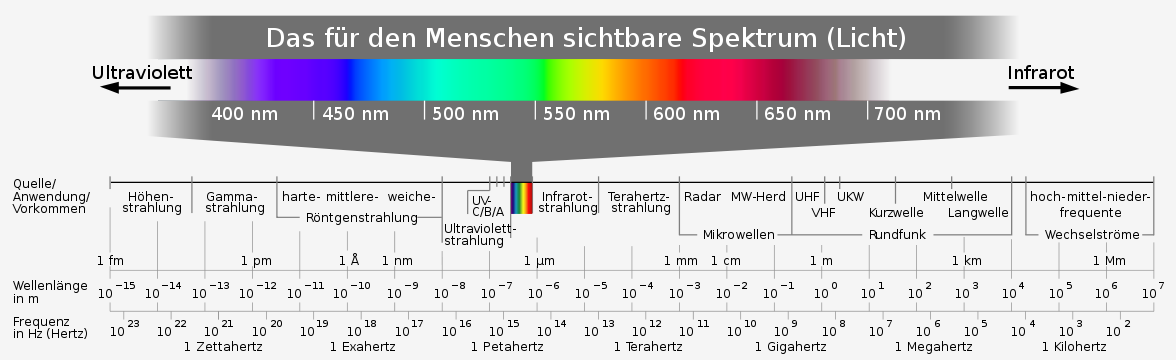
\includegraphics[width=\textwidth]{images/strahlung}

\begin{multicols}{2}
\paragraph {Lichtgeschwindigkeit im Vakuum}
$c = \frac {1}{\sqrt{\mu_0 \epsilon_0}} = 299792458 \frac{m}{s}$

\paragraph {Lichtgeschwindigkeit im Medium}
$c = \frac {1}{\sqrt{\mu_0 \mu_r \epsilon_0 \epsilon_r}}$ auf Leiterplatte $c = 20 \frac{cm}{ns}$ 
\end{multicols}

\paragraph {Photonen}
Licht besteht aus diskreten Energiequanten, den so genannten Photonen.
\begin{multicols}{3}
Energie: \\ $E = h * v$ \\
Plancksche Wirkungsquantum: \\ $h = 6.62606957 * 10^{-34} Js$ \\
Impuls: \\ $p = \frac {h}{\lambda}$ 
\end{multicols}

\subsubsection {Photoeffekt}
\begin{multicols}{4}
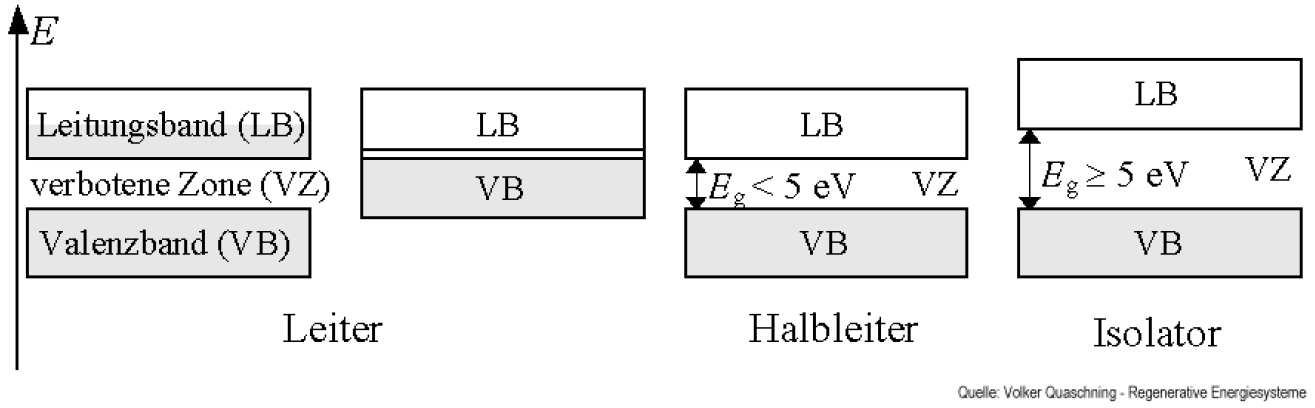
\includegraphics[width=0.5\textwidth]{images/Leitungsband} \\ \columnbreak 
\ \\ \vfill \columnbreak 
Mit der Energie des Lichtes kann ein Elektron auf eine höhere Bahn gehoben werden oder auch herausgeschlagen werden. \\ 
$E = \frac{h * c}{\lambda}$
\end{multicols}

\paragraph{äusserer Photoelektrischer Effekt}
Herauslösen von Elektronen aus einer Halbleiter- oder Metalloberfläche, benötigt eine hohe Ionisationsenergie.

\paragraph{innerer Photoelektrischer Effekt}
Silizium weist eine Bandlücke von 1.1eV auf zwischen dem Leitungs- und dem Valenz-Band. Damit ein Elektron den Sprung ins Leitungsband schafft, muss es die Energie von mindestens 1.1eV aufnehmen. Hat ein Photon diese oder eine grössere Energie, kann eine Wechselwirkung auftreten: Das Photon wird absorbiert, das Elektron springt ins Leitungsband und ein Loch bleibt zurück. Trifft ein Photon mit geringerer Energie auf den Silizium-Kristall, gibt es keine Wechselwirkung und das Photon fliegt durch den Kristall hindurch. Weist das Photon eine höhere Energie auf, so wird es absorbiert und die überschüssige Energie verpufft.

\paragraph{Photoleitung}
Erhöhung der elektrischen Leitfähigkeit von Halbleitermaterialien aufgrund der Bildung von ungebundenen Elektron-Loch-Paaren bei Bestrahlung. Die Elektronen werden vom Valenzband in das energetisch höher gelegene Leitungsband gehoben.

\paragraph{photovoltaischerEffekt}
Ladungsträgerpaare, die in der Raumladungszone, also am p-n-Übergang einer Photodiode entstehen, werden in p-und n-Schicht getrennt. Die Elektronen gehen in die n-Schicht über, die Löcher in die p-Schicht. Es entsteht ein Photostrom gegen die Durchlassrichtung des p-n-Übergangs.

\begin{multicols}{2}
\subsection{Photometrie}
\subsubsection{Empfindlichkeit des Auges}
Bei einer Wellenlänge von 555 nm, einer gelb-grünen Spektralfarbe entsprechend, ist das Auge am empfindlichsten. Bei etwa 510 nm (grün) auf der einen Seite, und bei etwa 610 nm (orangerot) auf der anderen Seite des Maximums erreicht das Auge nur noch die halbe Empfindlichkeit. Bei 665 nm, der Farbe typischer roter Leuchtdioden, beträgt die Empfindlichkeit nur 4,5 Prozent derjenigen bei 555 nm. Bei etwa 380 nm (violett) bzw. 780 nm (tiefrot) ist die Empfindlichkeit fast Null. \\ \\
Der in Watt gemessene Strahlungsstrom muss mit der wellenlängenabhängigen Empfindlichkeitskurve des Auges gewichtet werden, um aus der physikalischen Lichtleistung ein quantitatives Mass für den im Auge erzeugten Lichtreiz zu erhalten.
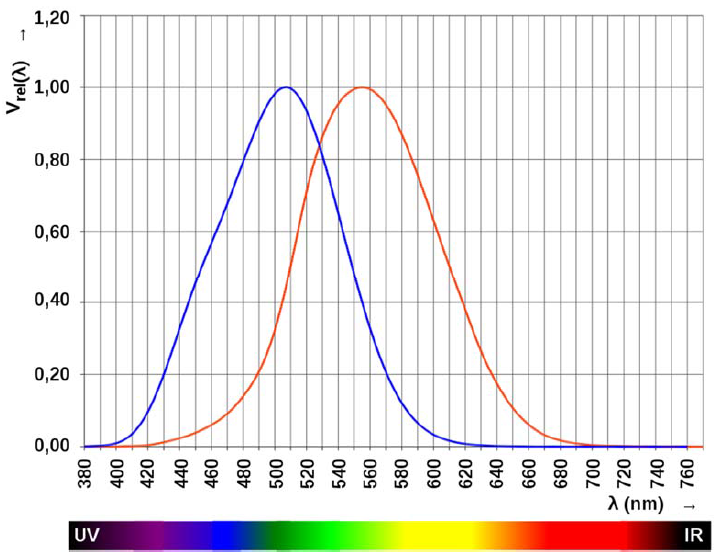
\includegraphics[width=0.5\textwidth]{images/empfindlichkeit_auge} 
\end{multicols}

\subsubsection{Photometrische Grössen}
An sich könnten für die Messung der Lichtstrahlung die normalen physikalischen Grössen und Einheiten verwendet werden. Um jedoch die spektrale Empfindlichkeit des menschlichen Auges zu berücksichtigen, werden spezielle lichttechnische Grössen und Einheiten eingeführt. Das gewichtete Mass wird in Lumen gemessen, die physikalische Leistung in Watt.

\subsubsection{Photometrisches Strahlungsäquivalent einer Strahlung}
Das Verhältnis des resultierenden Lichtstroms zur physikalischen Strahlungsleistung ist das photometrische
Strahlungsäquivalent der betreffenden Strahlung. Das Wellenlängengemisch des Tageslichts (ohne direkte Sonnenstrahlung) hat beispielsweise ein photometrisches Strahlungsäquivalent von etwa 125 $\frac{lm}{W}$, das der Sonne liegt zwischen knapp 20 $\frac{lm}{W}$ (tiefstehende Sonne)und etwa 100 $\frac{lm}{W}$ (Sonne im Zenit). Aus der Neudefinition der Einheit Candela (1979) folgt, dass monochromatische Strahlung der Frequenz 540*1012 Hertz (entspricht in Luft der Wellenlänge 555 nm) und der Strahlungsleistung 1 Watt gleichzeitig ein Lichtstrom von 683 Lumen ist. Die Strahlungsleistung auf anderen Wellenlängen trägt geringer zum Lichtstrom bei.

\subsubsection{Lichtausbeute einer Lichtquelle}
Das in $\frac{lm}{W}$ gemessene photometrische Strahlungsäquivalent ist nicht zu verwechseln mit der ebenfalls in $\frac{lm}{W}$ gemessenen Lichtausbeute einer technischen Lichtquelle. Das photometrische Strahlungsäquivalent beschreibt, wie viel abgegebenes Lumen auf jedes Watt der abgegebenen elektromagnetischen Strahlungsleistung entfallen. Die Lichtausbeute beschreibt, wie viel abgegebenes Lumen auf jedes Watt der von der Lichtquelle aufgenommenen (meist elektrischen) Leistung entfallen, schliesst also technische Umwandlungsverluste mit ein.

\subsubsection{Strahlungsstrom und Lichtstrom}
Die Strahlungsleistung wird Strahlungsstrom oder Strahlungsfluss genannt und mit $\Phi_e$ bezeichnet. Die entsprechende lichttechnische Grösse $\Phi_v$ wird Lichtstrom genannt. Die Einheit dafür ist Watt. \\
Ein Lumen ist der Lichtstrom, der durch eine Lichtquelle mit einer gleichmässigen Lichtstärke von einer Candela innerhalb eines Raumwinkels von einem Steradiant ausgestrahlt wird.

\subsubsection{Bestrahlungsstärke und Beleuchtungsstärke}
Die auf eine Oberfläche pro Flächeneinheit einfallende Strahlungsleistung wird Bestrahlungsstärke
genannt und mit $E_e$ bezeichnet. Die Einheit dafür ist $Wm^{-2}$. \\
Das Lux (Einheit $lx$) ist die SI-Einheit der Beleuchtungsstärke. Entsprechend ist die Beleuchtungsstärke der pro Flächeneinheit einfallende Lichtstrom. Sie wird mit $E_v$ bezeichnet und hat die Einheit $\frac{lm}{m^{-2}}$.

\subsubsection{Übersicht}
\begin{tabular}{|l|l|l|l|l|l|}
    \hline
    \multicolumn{3}{|l|}{Strahlungsphysikalische Grössen} & \multicolumn{3}{l|}{Lichttechnische Grössen} \\ \hline
    Grösse             & Symbol   & Einheit          & Grösse             & Symbol & Einheit      \\ \hline
    Strahlungsstrom    & $\Phi_e$ & $W$              & Lichtstrom         & $\Phi_v$ & $lm$       \\ \hline
    Strahlstärke       & $I_e$    & $Wsr^{-1}$       & Lichtstärke        & $I_v$    & $cd$       \\ \hline
    Strahldichte       & $L_e$    & $Wm^{-2}sr^{-1}$ & Leuchtdichte       & $L_v$    & $cdm^{-2}$ \\ \hline
    Bestrahlungsstärke & $E_e$    & $Wm^{-2}$        & Beleuchtungsstärke & $E_v$    & $lx$       \\ \hline
\end{tabular}